\chapter{ %Memory Observable Injectable  Startable Trace 
MOIST simulations and semantics of CompCert}\label{ch:compcert}

The simple code in \autoref{example:remember} communicates with its environment in two main ways: (1) it takes an address as input and (2) reads from and writes to this location to increment the value stored there.
\begin{figure}\begin{lstlisting}[language=C, numbers=left]
int *buff;
void remember(int *p){
    buff = p;
}
void incr(void){
    ++(* buff);
}
\end{lstlisting}
\caption[Code example: \Ccode{remember} and \Ccode{incr}]{The function \Ccode{remember} records the address of some buffer, and \Ccode{incr} increments it by one. }
\label{example:remember}
\end{figure}
We will see how the specification of CompCert prevents us from reasoning about such programs, either as compilation units or as external functions, and we will show how to extend the specification of a compiler to lift these limitations.

First, CompCert can't give any guarantees about compiling the code in \autoref{example:remember} because it is not a complete program. It is reasonable to expect that the function \Ccode{remember} runs safely, given some assumptions (e.g. \Ccode{*p} is a valid address in memory). Unfortunately, CompCert's semantics assumes that a program starts executing with a call to  \Ccode{main()} with no arguments. CompCert characterizes the initial state by a predicate \Coqcode{initial_state: state -> Prop} that takes no additional arguments. You can see an instantiation of the predicate for Clight in \autoref{code:initial_state}. So, even though CompCert correctly compiles the code, its specification gives no guarantees of any execution other than the one that starts by calling main with no arguments.
\begin{figure}
\begin{lstlisting}
Inductive initial_state (p: program): state -> Prop :=
  | initial_state_intro: forall b f m0,
      let ge := Genv.globalenv p in
      Genv.init_mem p = Some m0 ->
      Genv.find_symbol ge p.(prog_main) = Some b ->
      Genv.find_funct_ptr ge b = Some f ->
      type_of_fundef f = Tfunction Tnil type_int32s cc_default ->
      initial_state p (Callstate f nil Kstop m0).
\end{lstlisting}
\caption[\Ccode{initial_state} predicate for C]{The \Ccode{initial_state} in C and Clight describes a call to \Ccode{main}. It also enforces that it takes no arguments (\Coqcode{Tnil}) and returns an integer (\Coqcode{ type_int32s}).}\label{code:initial_state}
\end{figure}

Second, imagine that the example in \autoref{example:remember} describes not the program being compiled but the semantics of two system calls \textsf{remember} and \textsf{incr}.  Suppose CompCert compiles some program that calls \Ccode{incr()}; then the compiler's specification gives no guarantee about the behavior of the compiled code. Indeed, CompCert's semantics allows calls to external functions that are assumed to be correct but, unfortunately, that specification of correctness is too strict; it  assumes that the function's behavior is fully determined by (1) the state of memory, (2) the function arguments and (3) the events produced by the function.\footnote{Leroy \cite{Leroy-Compcert-CACM} claims that ``inputs given to the programs are uniquely determined by their previous outputs", but this is not exactly correct. A more accurate representation of CompCert?s specification would be to say ``inputs given to the programs are uniquely determined by their most recent outputs". Indeed, the semantics of external calls \Coqcode{extcall_sem : Type :=  env -> list val -> mem -> trace -> val -> mem -> Prop} are determined by the environment, the arguments to the call, the current memory and produce a trace, a return value and a return memory. As we will see in \autoref{sec:compcert-sim}, it would be much stronger to determine inputs based on all historic outputs.} The behavior of \Ccode{incr} also depends on the value in \Ccode{buff} (which for system calls will not be in the program's accessible memory), so it is not correct, according to CompCert's specification. Certainly, \Ccode{incr} could expose the pointer stored in \Ccode{buff} as part of its trace but CompCert events, shown in \autoref{code:oldevents}, can only contain integers, floats or pointers to global variables.
 
\begin{figure}\centering
\begin{multicols}{2}
\begin{lstlisting}[style=CoqTheorem-list]
Inductive event: Type :=
  | Event_syscall: 
  	string -> list eventval -> 
  	eventval -> event
  | Event_vload: 
  	memory_chunk -> ident -> 
  	ptrofs -> eventval -> event
  | Event_vstore: 
  	memory_chunk -> ident -> 
  	ptrofs -> eventval -> event
  | Event_annot: 
  	string -> list eventval -> event
  \end{lstlisting}
  \columnbreak
  \begin{lstlisting}
Inductive eventval: Type :=
  | EVint: int -> eventval
  | EVlong: int64 -> eventval
  | EVfloat: float -> eventval
  | EVsingle: float32 -> eventval
  | EVptr_global: ident -> ptrofs -> eventval.
  \end{lstlisting}
\end{multicols}
\caption[Events in CompCert]{The events in CompCert}\label{code:oldevents}
\end{figure}

Moreover, in the CompCert semantics, the entire behavior of each external function call is bundled into one big step. Looking at an execution, internal steps and external function calls are uniform. This consistency is very useful when reasoning about the compilation of the program, where we want to abstract external calls. Nevertheless, when reasoning about a program in a context, it is more useful to replace the big step external calls with their small step semantics. Regrettably, the specification of CompCert does not even guarantee that the source and target programs call the same external functions. In theory, CompCert could replace an external function call with internal steps as long as they had the same (possibly empty) trace. In practice, obviously, CompCert does not do that, this guarantee is not exposed in its specification.

Finally, the correctness of CompCert is stated as a semantic preservation theorem, where the traces are the preserved behavior and the proof uses forward simulations\footnote{Forward simulation and determinism of the target language implies bisimulation and thus preservation of behavior.}. At least two other works (\cite{compcomp}, \cite{jiang14:pldi}) have proposed alternative CompCert specifications that make the simulations an exposed feature of the compiler's specification. In these papers, the authors view CompCert correctness modularly as a thread-local or module-local simulation and recover a simulation of the global program later. Moreover, from the exposed simulations, they can recover the relation between memories in source and target, another very useful feature in compositional compilers, which seems to be a key feature in compositionally. Following this line of work, we propose to expose the simulation as the specification of the compiler, deriving semantic preservation as a corollary. 

Finally, in each CompCert intermediate language, every state of the small-step semantics contains exactly one memory.  To reason parametrically about how a thread of execution evolves its memory, we need a uniform way to access the memory component of the small-step state.
 
We move, then, to lift these limitations according to the following richer notion of specification:
\begin{definition}[MOIST simulations]
We say that a compiler's specification uses Memory, Observable, Injectable and Startable Trace (MOIST) simulations if they satisfy the following:
\begin{itemize}
\item Memory: All intermediate languages have a unified memory model \Coqcode{mem}, and each language $L_1$ has a function \Coqcode{get_mem: state L\_1 -> mem}, that exposes the memory of a state. The simulation describes the relation between memories before and after compilation.  
\item Observable: Similarly, all intermediate languages are outfitted with a function \Coqcode{at_external} that identifies states about to make an external function call. For every language $L_1$, \Coqcode{at_external: state L_1 -> option (f_ext, args)} returns the external function being called and its arguments. The simulation preserves external calls. 
\item Injectable: The execution trace supports events that can describe locations in memory (i.e., pointers). Compilation may rearrange memory, which CompCert describes as an \emph{injection}, so the trace will be preserved up to these injections. The simulation shows that the injection relating traces in source and target executions is the same injection that relates their memory. We call these new events \emph{memory events}.
\item Startable: The execution of a program can start in any of its public functions, including \Ccode{main}, taking arguments.  

%\item The correctness of the compiler is stated as a forward simulation and the semantic preservation derive as a corollary. The forward simulations preserve external function calls and exposes the relation between source and target memories, throughout the execution. We call this an \emph{exposed simulation}. 
\end{itemize}
\end{definition}
It is worth noting that, even though we require a unified memory model, in practice, a language can use a different memory model (or none at all) as long as it can construct a memory from its state with \Coqcode{get_mem}. In practice all CompCert languages use the same memory model, described in \autoref{sec:compcert-mem}, which we will refer to as \Coqcode{mem} from now on.
Nevertheless, a future language could use \emph{juicy memory} as in \cite{appel14:plcc} or abstract state in \cite{Ronghui15abstractionlayers} since a \Coqcode{mem} can be derived from them. 

\def\percchange{3.6\%}
\begin{table}
\centering
\begin{tabular}{|c|c|c|} \hline  
		& Percent change & Number of lines changed \\
\hline Arguments in \Ccode{main} & 1.6\% & 3660 \\ %Calculated as diff, to when entry_points branch started: gif diff --stat ff3f7c830c7676f7847ca9391d2786da3236c9f6
\hline Injectable Traces & 0.5\% & 1141 \\  %use [ git diff --stat f047fcb7852ff58c0c62f10d41f91f3f88552780] and look changes in [Events.v + EventsAux.v]
\hline MOIST Semantics & 0.2\% & 466 \\  % [387 = 43 * 9 + 79] calculated as number of lines to define a new semantics * number of languages. + new deifnitions of semantics.
\hline MOIST Simulations & 1.3\% & 2911 \\ % The rest: = 8178 - 466 - 1141 - 3660 - 2911
\hline \textbf{Total} & \percchange & 8178 \\ %total computed with  git diff --stat f047fcb7852ff58c0c62f10d41f91f3f88552780. Removing the lines from Driver/compiler.v
\hline \end{tabular}
\caption[Measures of changes to CompCert.]{Measures of changes to CompCert: changes are calculated from the number of lines added as given by running \Ccode{git diff} between our code and the commit of CompCert we branched off from. For each feature, an estimated number of lines is provided. }\label{tab:prcntchange}
\end{table}

In the rest of the chapter, we describe how we develop MOIST specifications for CompCert. We first describe how to generalize \Coqcode{initial_state} to make the simulations Startable. Second we describe how to add memory events to CompCert. Then we show how to extend the semantics for every language in CompCert to include \Ccode{get_mem} and \Coqcode{at_external} functions and, finally, we show how to put everything together in MOIST simulations for CompCert, which proves the following theorem:

\begin{theorem}[CompCert MOIST specification]\label{thm:moistsim}
Given a source program P and an x86 assembly language program Q obtained by CompCert compilation of P, the CPMs of the two programs are in a MOIST simulation relation.
\end{theorem}
  

The changes described here represent only a \percchange\ %TODO
change to CompCert, as measured by running \Coqcode{git diff} in CompCert before and after our changes. The amount changed for every feature proposed is described in \autoref{tab:prcntchange}.\footnote{All these measurements are made with respect to a commit in CompCert from May 21 (\Ccode{f047fcb7852ff58c0c62f10d41f91f3f88552780})}
Approximately 10\% of all new additions are specifications and the rest are proofs. 

\section{Memory model and memory injections}\label{sec:compcert-mem}

All intermediate languages in \compcert\ use the same memory model \cite{Leroy-Blazy-memory-model}. This is a key feature of the CompCert's proof of correctness, since it facilitates reasoning about how the compiler lays out stack frames in memory. In this section we briefly describe the memory model and the \emph{memory injections} which describe the evolution of the memories (particularly stack frames) through compilation.


\begin{figure}
$$\begin{array}{rccl} 
&\text{block}& ::= & \mathbb{N} \\
\text{Blocks} &  b & ::= &\text{block} \\
\text{Offsets} & ofs & ::= & \mathbb{Z} \\
\text{Values} & v & ::= & \text{Vundef} \ |\  \text{Vint}\ n \ |\  \text{Vfloat}\ n \ |\  \text{Vptr}\ b\ ofs \\
\text{mem} & m & \in & \mathbb{N} \rightarrow \text{option} (\mathbb{N} * \mathbb{Z}) \\
\text{perm} & p & ::= & \text{None} \ |\  \text{Nonempty} \ |\  \text{Readable} \ |\  \text{Writable} \ |\  \text{Freeable} \\
\text{Max perm} & \text{Max} & \in & \text{mem}\rightarrow (\text{block} * \mathbb{Z}) \rightarrow \text{Perm} \\
\text{Cur perm} & \text{Cur} & \in & \text{mem}\rightarrow (\text{block} * \mathbb{Z}) \rightarrow \text{Perm} \\
\text{injection}& j& \in & \text{block} \rightarrow \text{option} (\text{block} * \mathbb{Z})\\
\end{array}$$
\caption{\compcert\ memory model.}
\end{figure}
CompCert's memory is represented by a two dimensional array of bytes, indexed by a block reference and an integer offset. Each single block is a one dimensional array that can be used differently for each intermediate language; in Clight, every stack-allocated variable is in a separate block while in Mach every stackframe sits in a single block. The bytes in each location are represented by abstract values such as integers, floats, pointers; or undefined, if its location has not been initialized. 
  
Every location in memory is also outfitted with permissions that regulate how a program can interact with memory. These permissions are cumulative, so each one grants the capabilities of all the permissions below:

\begin{tabular}{rl} 
Freeable: & can free the location \\
Writable: & can write to the location\\
Readable: & can read to the location\\
Nonempty: & can only compare pointers to the given location\\
None: & Can't interact with the location\\
\end{tabular}

For example, a program may only free a piece of memory if it has \Coqcode{Freeable} permission of that location; but it can read any location where it has at least \Coqcode{Readable} permission. 
It is intended that a thread may gain or lose permissions to a location by doing synchronizations such as acquire and release; to keep track of this, there is a \Coqcode{Cur} (current) permission at each address.  But to prove the correctness of a certain optimization (constant-folding the load of a global read-only variable), the semantics also has a \Coqcode{Max} permission at each address, above which Cur can never go.
For example, all global variables have at most \Coqcode{Writable Max}  permissions so they might change, but they can't be freed. \Coqcode{Cur} permissions represent local abilities of a module or thread. For example, a thread will have no permissions for variables in the stack of another thread, whose addresses are not taken. But no matter how much more \Coqcode{Cur} permission a thread gains by acquiring a lock (etc.), it can never go above the \Coqcode{Max} permission for the address.

The compiler must preserve the behavior of a compiling program, but it might reorder and change its accesses to memory; an optimization might swap two consecutive memory allocations, or it might add new ones during spilling. Even so, the memory can't change too much, lest it change the observable behavior of the program. In the CompCert memory model, the compiler can affect memory blocks by reordering them, deleting them, changing their internal offsets or even merging two of them. Leroy and Blazy \cite{Leroy-Blazy-memory-model} call these transformations \emph{memory injections} and, to prove memory-changing optimizations are correct, they show that the observable behavior of a correct program is invariant under memory injections. We will describe injections further below.

Most \compcert\ passes don't change the memory behavior of the program. For example, the phase Cshmgen simplifies control structures, but preserves all memory accesses. In that way, the executions of the program before and after the pass display the same memories at every point. These are \emph{equality passes}. Some passes might increase the size of a block by, for example, spilling variables to the stack, but won't reorder the blocks; we call these  \emph{extension passes} \autoref{fig:memtransforms}(b). Finally there are those that delete, reorder and merge blocks, such as the Csharpminor to Cminor pass which merges all stack-allocated variables into  single block (the stack block). These are the \emph{injection passes}\ \autoref{fig:memtransforms}(a). All passes can be shown to be injections \cite{compcomp}, but it is much easier to treat equality and extension phases as special cases. 

\begin{figure}
\begin{multicols}{2}
~~\raisebox{4ex}{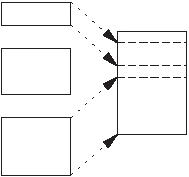
\includegraphics[height=90pt]{graphics/memfig3a.pdf}}

(a) Memory injection

\columnbreak
~~\raisebox{4ex}{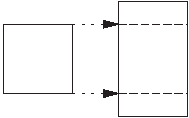
\includegraphics[height=90pt]{graphics/memfig3b.pdf}}

(b) Memory extension

%\columnbreak
%
%Equality diagram
%
%(c) Memory equality
\end{multicols}
\caption[Memory transformations of CompCert]{Memory transformations of CompCert. \cite{appel14:plcc}  }\label{fig:memtransforms}
\end{figure}

% More about injections
An injection is described by a mapping $j:$ \Coqcode{block -> option (block * Z)}, that determines if a block is mapped and, if so, to which block and with what offset. For example in the Csharpminor to Cminor pass, where local variables are coalesced into one stack block, each variable will be offset such that it doesn't overlap with the others as shown in \autoref{fig:memtransforms}(a). Beyond a permutation of memory, an injection induces relations between the source and target contents of memory and the permissions. We abuse the notation $\overset{j}{\hookrightarrow}$ to denote all these relations induced by injections, including several others we define in the following sections. 


\def\ofs{i} 

 \begin{figure}\centering
 %\begin{multicols}{2}

\fbox{
\begin{mathpar}
\inference{}{\mathsf{Vint}(n) \strinjarrow{j} \mathsf{Vint}(n)}
\and
\inference{}{\mathsf{Vfloat}(n) \strinjarrow{j} \mathsf{Vfloat}(n)}
\and
\inference{F(b_1) = \text{Some}\ (b_2, \delta) & \ofs_2 = \ofs_1 + \delta}{
\mathsf{Vptr}(b_1,\ofs_1) \strinjarrow{j} \mathsf{Vptr}(b_2,\ofs_2)}
\and
\inference{v_1 \strinjarrow{j} v_2}{v_1 \injarrow{j} v_2}
\and
\inference{}{\mathsf{Vundef}\injarrow{j} v_2}
\end{mathpar}
}
(a) Strong ($\strinjarrow{}$) and simpl ($\injarrow{}$) value injections.

%\columnbreak

\fbox{\begin{mathpar}
\inference{}{p \injarrow{j} p}
\and
\inference{}{\mathsf{None}\injarrow{j} \mathsf{Freeable}}
\end{mathpar}
}

(b) Permission injections

%\end{multicols}
\caption{Value and permission injections}\label{fig:valueinj_perminj}
\end{figure}

An injection imposes a relation between values before and after the compiler pass, as described in \autoref{fig:valueinj_perminj}(a). In the stronger injection, constants are preserved and pointers are renamed according to the injection. In the simpl injection, undefined values are also allowed to map to any concrete value because, in compiler passes such as register coalescing, uninitialized local variables, can map to initialized ones with concrete values. Similarly, the injection imposes a relation between permissions as shown in  \autoref{fig:valueinj_perminj}(b).


\begin{definition}[memory injection]\footnote{We omit a couple extra properties such as \emph{not overlapping} and \emph{memory alignment}.} Two memories $m_1$ and $m_2$ are \emph{injected} by $j$ ($m_1 \injarrow{j} m_2 $) if, for all locations $b_1$ mapped by $j \ b_1 = \text{Some}\ (b_2, \text{ofs})$ :
\begin{itemize}
\item Permissions are injected on all offsets $x$: 
$$\text{Max}\ m_1\ (b_1,\ x)  \injarrow{j} \text{Max}\ m_2\ (b_2,\ x + \text{ofs}) \ \ \ \text{and}$$ $$\text{Cur}\ m_1\ (b_1,\ x)  \injarrow{j} \text{Cur}\ m_2 (b_2,\ x + \text{ofs})$$

\item Values are injected on all visible offsets $x$: 
$$\text{Cur}\ m_1\ (b_1,\ x)  \geq \text{Readable} \rightarrow m_1\ (b_1,\ x)  \injarrow{j} m_2\ (b_2,\ x + \text{ofs})$$

\item Only allocated blocks are mapped and the image of mapped blocks don't overlap.

\item \Coqcode{mi_representable} and \Coqcode{mi_perm_inv} \cite{appel14:plcc}  

\end{itemize}
\end{definition}







   

\section{Passing arguments to main.}\label{sec:premain}

CompCert can compile programs where \Ccode{main} takes arguments, but its correctness theorem gives no guarantees about their translation. That is because it's semantic model assumes that \Ccode{main} takes no arguments (See \ref{code:initial_state}), but real C programs can take up to two arguments \Ccode{argc} (argument count) and \Ccode{argv} (argument vector). Also, all execution is the semantics of CompCert start with a call to \Ccode{main()}, but \Ccode{main} is nothing but an agreed upon term for startup code. Furthermore, the semantics assumes that the initial memory contains only the global environments. In this section we define a new predicate \Coqcode{entry_point}, generalizing \Coqcode{initial_state}, which accepts any public function, including those with arguments. The predicate also admits other memories containing, for example, the stack of other processes. 

Passing arguments to main is of general interest and particularly important for our work with concurrency. Spawning new threads behaves very similar to starting a program by calling \Ccode{main}: The library function that spawns a new thread \Ccode{f} (e.g. \Ccode{pthread_create}) must create a new stack, push the arguments to stack and then call \Ccode{f} just like a program startup (which calls \Ccode{_start()} and \Ccode{__libc_start_main()}). Our new predicate \Coqcode{entry_point} is general enough to capture this two types of preprocessing.
Notice that if we restricted our semantics to spawning threads whit no arguments, threads wouldn't be able to share pointers and thus they would all execute in disjoint pieces of memory with no communication. That would be a much easier and less interesting result. 

Now that we defined a new starting point for executions, we must prove that compilation preserves the predicate \Coqcode{entry_point} in the same way that CompCert's simluation preserves \Coqcode{initial_state}. The proof largely follows the simulation of internal function calls which is already proven in CompCert, so we omit the details here. 

\begin{table}\centering
\begin{multicols}{2}\begin{tikzcd}[column sep=tiny]
 \arrow[d, "\text{initial\_state}"']
&  &  \arrow[d, dotted,  "\text{initial\_state}"] \\
s_1 & \widesim{} & s_2
\end{tikzcd}

(a)

\begin{tikzcd}[column sep=tiny]
\arrow[d, "\text{entry\_points } m_0 \ f \ \text{args}"']
&  &  \arrow[d, dotted,  "\text{entry\_points } m_0 \ f \ \text{args}"] \\
s_1 & \widesim{} & s_2
\end{tikzcd}

(b)
\end{multicols}
\caption{Entry simulation diagrams. (a) if $s_1$ is an initial state for the source program, then there exists some state $s_2$ that is related to $s_1$ and is an initial state for the compiled program. (b) Just like the diagram for initial states, but it generalizes and exposes the initial memory $m_0$, the entry function $f$ and the arguments \Coqcode{args}. The entire simulation is parametric on the realation $\sim$.}\label{table:initial_sim}
\end{table}

\subsection{Simulating initialization preprocessing.}
Before \Ccode{main} ever starts executing, there is an initialization process that sets up the stack and the registers, before main is executed. The preprocessing function(s) often called \Ccode{_start}, \Ccode{premain} or \Ccode{startup}, will create a stack, set up the arguments in the stack or in registers, set up the environment (\Ccode{envp}), set up the return address (a call to \Ccode{exit()}), and other bookkeeping. 


One of the difficulty in simulating the initialization is that, in architectures such as $x86$ in $32$-bit mode, all arguments are passed in memory. As the comments in the CompCert code would put it "Snif!"\cite{leroy19:compcert}. Even architectures that allow argument passing in registers, such as $x86$ in $64$-bit mode, have a limited number of registers and will pass arguments on the stack after those run out. This "pre-stack", that contains the arguments, does not correspond to any function in the call stack of the program; it corresponds to the stack frame of \Ccode{_start()}, which is part of the linked program.

Our generic predicate \Coqcode{entry_points: mem -> state -> val -> list val -> Prop} takes a memory \Coqcode{m}, a state \Coqcode{s}, a pointer to the entry function \Coqcode{fun_ptr} of type \Coqcode{val}, and a list of arguments \Coqcode{args}. This predicate is language dependent, but it generally has three parts:
\begin{enumerate}
\item Checks memory is well formed. That is, it contains no ill-formed pointers to invalid memory. CompCert generally maintains that well formed programs don't create dangling pointers pointers.\footnote{A well formed program, should not compare, read or write to invalid pointers. Hence, dangling pointers behave semantically as undefined values and could be modeled that way.}
\item Arguments are well formed. Among other things, they have the right types for the function being called, they have no ill-formed pointers, and fit in the stack. 
\item Global environment is allocated correctly. This makes sure that the environment is in memory and that the function is declared as a public in the environment.
\end{enumerate}
In the rest of this section, we explore the definition of \Coqcode{entry_points} for different languages and show how we prove that different CompCert phases preserve the predicate.

\subsubsection{C frontend}
All of the C-like languages (\emph{Clight, Csharp, Csharpminor}) have similar \Coqcode{entry_point}, so we present here the one for Clight in \ref{code:entry_point_Clight}.
\lstset{moredelim=*[s][\color{green}]{Inductive}{' '}}
\begin{table}
\begin{lstlisting}[ numbers=left]
Inductive entry_point (ge:genv): mem -> state -> val -> list val -> Prop :=
| initi_core: forall f fb m0 args targs,
      let sg:= signature_of_type targs type_int32s cc_default in
      type_of_fundef (Internal f) = Tfunction targs type_int32s cc_default ->
      Genv.find_funct_ptr ge fb = Some (Internal f) ->
      globals_not_fresh ge m0 ->
      Mem.mem_wd m0 ->
      Val.has_type_list args (typlist_of_typelist targs) ->
      vars_have_type (fn_vars f) targs ->
      vals_have_type args targs ->
      Mem.arg_well_formed args m0 ->
      bounded_args sg ->
      entry_point ge m0 (Callstate (Internal f) args (Kstop targs) m0).
\end{lstlisting}
\caption{The \Ccode{entry_point} predicate in Clight}\label{code:entry_point_Clight}
\end{table}
Lines 4-6 ensure that the environment is allocated in memory and it contains the function \Coqcode{f} with the right type signature. Line 7 states that the initial memory has no dangling pointers. Lines 8-11 say that the arguments have the right type and have no dangling pointers. The predicate \Coqcode{bounded-args}, enforces that the arguments fit in the stack, which is architecture dependent. It is reasonable to replace this with a small enough bound that fits all architectures, like $4$, but we keep it general here. Finally, the entry state, in line 13, is defined as a call to \Coqcode{f} with an empty continuation.

Our empty continuation \Coqcode{Kstop} takes \Coqcode{targs} as an arguemnt. That is because continuations also represent the call stack; \Coqcode{Kstop targs} represents the "pre-stack" of \Ccode{_start()} that might contain some arguments for \Coqcode{f}.

\subsubsection{Register transfer languages}
In the Cminorgen phase, CompCert coalesces  all function variables into a stackframe. Some functions might get empty stackframes (i.e., a memory block with empty permissions, that cannot be written to), if none of their variables has their address taken. These stackframes are important, even the empty ones, because that is where spill variables will be written after register allocation in the Allocation phase. We follow suit and create an empty stackframe for \Ccode{_start()}. The stack is empty because the compiler has not yet decided what arguments will be passed in memory and which ones in register. Even for architectures that pass all arguments in memory, this is not doesn't until the Stacking pass. So for languages before Stacking (Cminor, CminorSel, RTL, LTL, Linear), there is an extra line in \Coqcode{entry_point} to make sure that the empty stackframe is allocated:
\begin{lstlisting}
	Mem.alloc m0 0 0 = (m1, stk) \end{lstlisting}
The rest of the predicate is almost identical to the one in \ref{code:entry_point_Clight}.

\subsubsection{Machine languages}

In the machine languages (Mach and Asm), a function expects certain shape from the stackframe of its caller. We replace the empty stackframe allocation above, with the constructon of the "pre-stackframe" as shown in \ref{code:entry_point_Mach}.
\begin{table}
\begin{lstlisting}[ numbers=left]
      $\vdots$
      let '(stk_sz,ret_ofs,parent_ofs) := stack_defs (fn_sig f) in
      Mem.alloc m0 0 stk_sz = (m1, spb) ->
      let sp:= Vptr spb Ptrofs.zero in
      store_stack m1 sp Tptr parent_ofs Vnullptr = Some m2 ->
      store_stack m2 sp Tptr ret_ofs Vnullptr = Some m3 ->
      make_arguments (Regmap.init Vundef) m3 sp
                     (loc_arguments (funsig (Internal f))) args = Some (rs, m4) ->
      $\vdots$
\end{lstlisting}
\caption{Part of the \Ccode{entry_point} predicate in Mach}\label{code:entry_point_Mach}
\end{table}
The function \Coqcode{stack-defs} is an architecture dependent function that calculates the layout of the "pre-stack" and returns the size \Coqcode{stk_sz}, the ofset of the return address \Coqcode{ret_ofs} and a back link to parent frame \Coqcode{parent_ofs}. The last two values are unused, but the stack must have space for them. Line 3 allocates the stack of the correct size. Lines 5-8 store the return address, the link to the parent and the arguments in the stack. 
\section{Memory events.}

The visible behavior of the CompCert semantics (for all languages) is a trace of events, as described in \ref{code:oldevents}. It records interactions with the outside world; for example, the results of a read system call will record a \Coqcode{Event_syscall} together with the name of the system call, its parameters, and its result. The only pointers that can appear in the trace are locations of global variable. As we explained above, these events are insufficient to capture the behavior of \Ccode{incr} in \ref{example:remember}. The events are also not sufficient to express any kind of behavior that depends on the memory. For example, a call to \Ccode{pthread_mutex_ulock(&l)} not only changes the state of the lock \Ccode{l}, conceptually it gives away control to the data in memory protected by \Ccode{l}. Such behavior that reveals locations in memory cannot be expressed in CompCert events that can't have pointers on them (except the location of global variables). More generally, these events are poorly suited to express any sort of shared memory interactions, such as concurrency or separated compilation. 
\begin{table}\centering
\begin{multicols}{2}
\begin{lstlisting}
Inductive event: Type :=
  $\cdots$
  | Event_acq_rel: 
  	list mem_effect -> 
	delta_perm_map -> 
	list mem_effect -> event
  | Event_spawn: 
  	block -> 
  	delta_perm_map -> 
  	delta_perm_map -> event.
	
  \end{lstlisting}

	
  \begin{lstlisting}
Inductive mem_effect: Type :=
|  Write : forall (b : block) (ofs : Z)
		(bytes : list memval), mem_effect
| Alloc: forall (b : block)(lo hi:Z), mem_effect
| Free: forall (l: list (block * Z * Z)), mem_effect.
  \end{lstlisting}
  
  \
	
	\
	
	\
	
\end{multicols}
\caption{The new events in CompCert:  \Coqcode{mem_effect} reflects changes to memory and \Coqcode{delta_perm_map} represents transfer of \Coqcode{Cur} permissions.}\label{code:newevents}
\end{table}
We propose to include 2 new types of events which we call \emph{memory events} as described in table \ref{code:newevents}. As their name suggests, they contain references to locations in memory, beyond the global variables.  
%Acquire release
The first one, \Coqcode{Event_acq_rel}, represents a generic memory interactions where the external function performs some arbitrary changes to memory, recorded by a list of \Coqcode{mem_effect}s, and transfers some permissions recorded by \Coqcode{delta_perm_map}. We find it convenient to split the effects on memory as those that happen before the changes in permissions and those that happen after. 
%Event spawn
The second one,  \Coqcode{Event_spawn}, represents the creation of a new thread or a new module. It records the function being called, as a block number, and the change in permissions by two \Coqcode{delta_perm_map}, one representing the permissions given and the other the starting permissions of a new thread/module.

The correctness of the CompCert compiler is formulated as a preservation of traces. However, if our traces contain memory events and the memory can be reordered by compilation, the trace must be reordered accordingly. Thus our new correctness will be formulated up to memory reordering as shown in \ref{sec:step_diagram_sim}. In fact, if a compiler pass (or passes) don't change the order of memory (such as equality and extension passes), then the trace is preserved and nothing changes in the simulation. If the pass changes the order of memory according to some $j$, then we need show that the source and target traces,$t$ and $t'$, are related by \Coqcode{inject_trace_strong j t t'} (denoted $t \overset{j'}{\hookrightarrow} t'$). That means that events in $t$ and $t'$ are identical except all memory locations are reordered according to $j$. To add this property, we need simulations to expose how they reorder memory. The full description of our new conjunctive simulation will be explained in section \ref{sec:compcert-sim}.


Compilers not only reorder memory, sometimes undefined values in the source program are mapped to concrete values in the target. Such mappings are useful in compiler passes such as register coalescing, where registers that were previously uninitialized, can now map to an initialized register with concrete values. The predicate \Coqcode{inject_trace_strong} always maps undefined values to undefined values. This is a reasonable restriction since inspecting undefined values is not an allowed behavior, so they shouldn't appear in the trace. However, if an application required traces with undefined values, we can still support that. It turns out that it is enough to prove that the execution with the \emph{strongly injected} trace is safe, and from it we can derive save executions for all traces that have some undefined values defined.

\section{Conjunctive Semantics}\label{sec:compcert-sem}

As described in the introduction, we need more expressive semantics to distinguish the current memory, during program execution, and the points where external functions are called. We call this expanded semantics \emph{conjunctive semantics} and it extends CompCert semantics with the following

\begin{table}
\begin{lstlisting}
Definition at_external (c: state) : option (external_function * list val) :=
  match c with
  | Callstate fd args k _ =>
      match fd with
      | External ef targs tres cc => if ef_inline ef then None else Some (ef, args)
      | _ => None
      end
  | _ => None
 end.
\end{lstlisting}
\caption{\Coqcode{at_external} definition for Clight. The function checks that 
(1) the current state is about to make a function call, 
(2) that the function is an External function and, 
(3) that the external function cannot be inlined (The compiler is allowed to inline specific functions such as \Ccode{memcpy} and certain builtins). }\label{code:atxClight}
\end{table}


\begin{itemize}
\item \Coqcode{get_mem} and \Coqcode{set_mem}: The state of every language in CompCert can be interpreted as a pair of a \emph{core} and a memory \cite{compcomp}. \Coqcode{get_mem} is the projection that returns the memory inside the state and \Coqcode{set_mem} changes the memory.
\item \Coqcode{entry_points}: This is a generalization of \Coqcode{initial_state}, as described in section \ref{sec:premain}.
\item  \Coqcode{at_external} : This function exposes when a program is about to call an external function and it returns the function and the arguments being passed. The instantiation for Clight is shown in table \ref{code:atxClight}.
\end{itemize}    

Our conjunctive semantics is very closely related to \emph{interaction semantics} \cite{compcomp} with two main differences. First, we don't need to define \Coqcode{after_external} for every language. Second, states that are \Coqcode{at_external} can take a step in the CompCert semantics; namely, the execution will continue by calling the external function. The CompCert semantics, in this case, represents the \emph{thread-local} view (or \emph{module-local}) , where external functions, other threads and modules are abstracted into oracles that execute in one step.\footnote{In CompCert the oracle, called \Coqcode{external_functions_sem}, is passed as a parameter to the correctness proof and gives the semantic of external functions.}. 

In fact, given a conjunctive semantics we can derive an interaction semantics, if only we define \Coqcode{after_external}. The step relation is constructed by removing steps from states that make external function calls, as described by \Coqcode{at_external}. 
\section{More revealing simulations}\label{sec:compcert-sim}

CompCert's compiler specification is stated as the following semantic preservation theorem

\begin{theorem}[CompCert semantic preservation]
Let $S$ be a source program and $C$ its compiled version. For all behaviors $B$ that don't go wrong, if $S$ has behavior $B$, then  
$C$ also has behavior $B$. In short:
\begin{equation}\forall B \not \in \text{Wrong}. \ S \Downarrow B \Rightarrow \ C \Downarrow B\label{eqn:compcertspec1}\end{equation}
\end{theorem}
Here, a behavior is a a trace and a termination or divergence. If a specification $spec$ is a function of behavior, then it also holds that CompCert preserves specifications in the sense that:
\begin{equation} S \models spec \Rightarrow C \models spec \end{equation}
Such specification fails to preserve richer notions of specification, such as the higher-order, separation logic specifications that can be proven on Clight programs by tools like \cite{DBLP:journals/jar/CaoBGDA18} or [?]%\cite{What's the other}
. Moreover, the high level specification in \ref{eqn:compcertspec1} is not well suited for modular reasoning to support shared memory concurrency or compositional compilation \cite{compcomp}. 

We consider that the simulations that CompCert uses to prove \ref{eqn:compcertspec1} are better suited for these purposes.
CompCert proves a forward simulation between its source and target executions which, together with the determinism of the target language, imply \ref{eqn:compcertspec1}. These simulations, encoded in the record \Coqcode{fsim_properties}, state that (1) public global variables and functions are preserved, (2) \Coqcode{initial_states} are preserved (\ref{table:initial_sim}), (3) \Coqcode{final_states} are preserved and (4) execution is preserved (\ref{table:step_sim}(a)). The simulations is parametric on a \emph{match relation}, noted as $\overset{ }{\sim}$, as an invariant of related states in source and target; the relation is established at initial states and preserved by the step simulation. 

\begin{table}\centering
\begin{multicols}{2}

\

\begin{tikzcd}[column sep=tiny]
s_1 \arrow[d, "t"']
& \widesim{} & s_2 \arrow[d, dotted,  "t"', "*"] \\
s_1' & \widesim{} & s_2'
\end{tikzcd}


\

(a)
\begin{multicols}{2}
\begin{tikzcd}[column sep=tiny]
s_1 \arrow[d, "t"']
& \widesim{j } & s_2 \arrow[d, dotted, "t'"',"*"] \\
s_1' & \widesim{j' } & s_2'
\end{tikzcd} 

$$t \overset{j'}{\hookrightarrow} t'$$
$$j \sqsubseteq j'$$
\end{multicols}

(b)
\end{multicols}
\caption{Step simulation step diagrams. (a) if $s_1$ takes a step to $s_2$ with trace $t$ and $s_1$ is related to some $s_2$, then there $s_2$ can take a number of steps with trace $t$ to a new state $2_2'$ related to $s_1'$. (b) The new diagram exposes the memory reordering injections $j$ and $j'$ and the traces $t$ and $t'$ are equivalent up to injection, by \Coqcode{inject_trace_strong j' t t'}. }\label{table:step_sim}
\end{table}
For all CompCert phases, the \emph{match state} relation describes how the memory changes after compilation. In some passes, memory doesn't change at all (e.g. Cshmgen or Linearize) and sometimes the memory is extended by increasing the size of existing memory blocks, with new values (e.g. Allocation, Tunneling). In other cases, memory is reordered, memory blocks are coalesced, and some are unmapped. CompCert expresses this reordering with \emph{memory injections} that map memory blocks, to their new block with some offset. For example, in Cminorgen the compiler coalesces all stack-allocate local variables of a function into a single stack block. We use this same injection to describe how traces with memory events evolve through compilation (\ref{table:step_sim}(b)).

We propose a more expressive simulation \Coqcode{inject_sim} that improves the CompCert simulations in the following ways:

\begin{itemize}
\item Exposes how the memory changes: We expose the memory injection $j$ that describes how memory changes after compilation. For simplicity of the proofs, for compiler passes that preserve the memory or just extend it, we also define the simpler simulations  \Coqcode{eq_sim} and \Coqcode{extend_sim} respecively. These simulation follow immediately from the ones already proven in CompCert. All of the simulations we define compose horizontally to \Coqcode{inject_sim} as shown by the composition lemmas \ref{lemma:eq_extend}, \ref{lemma:extend_inj} and \ref{lemma:inj_inj}.
%\begin{table}\centering
%\begin{lstlisting}[style=CoqTheorem-list]
%fsim_simulation:
%          forall s1 t s1' f, Step L1 s1 t s1' ->
%           forall i s2, match_states i f s1 s2 ->
%          exists i', exists s2' f' t',
%          (Plus L2 s2 t' s2' \/ (Star L2 s2 t' s2' /\ i' \leq i))
%          match_states i' f' s1' s2' /\
%          inject_incr f f' /\
%           inject_trace_strong f' t t'
%  \end{lstlisting}
%\caption{The new simulation step diagram}\label{code:sec:step_diagram_sim}
%\end{table}

\begin{lemma}\label{lemma:eq_extend}
For all semantics $L_1$ and $L_2$ if \Coqcode{eq_sim} $L_1 \ L_2$ then \Coqcode{extend_sim} $L_1 \ L_2$\end{lemma} 
\begin{lemma}\label{lemma:extend_inj}
For all semantics $L_1, L_2, L_3$, if \Coqcode{extend_sim} $L_1 \ L_2$ and \Coqcode{inject_sim} $L_2 \ L_3$, then \Coqcode{inject_sim} $L_1 \ L_3$
\end{lemma} 
\begin{lemma}\label{lemma:inj_inj}
For all semantics $L_1, L_2, L_3$, if \Coqcode{inject_sim} $L_1 \ L_2$ and \Coqcode{inject_sim} $L_2 \ L_3$, then \Coqcode{inject_sim} $L_1 \ L_3$
\end{lemma} 


\item Preserves external function calls: The original CompCert simulation only preserves traces so, for example, a compiler could replace an external function call with internal code that produces the same event. In fact the compiler does exactly that with some special external calls such as \Ccode{memcpy} and certain builtins. However the compiler does not do that with arbitrary external functions (of cours not!), but the simulation specification does not rule it out.  We add \Coqcode{preserves_atx} to the simulation, which says that if a source state is \Coqcode{at_external}, then any target state it matches is also \Coqcode{at_external} with the same functions and related arguments (i.e., equal up to memory injection).  

\item Preserves the number of steps taken by external functions: This fact was already proven in the CompCert but was hidden in the less expressive simulation. We include a new diagram (\ref{table:atx_sim}), \Coqcode{simulation_atx} which says that if a source state, that is \Coqcode{at_external} takes exactly one step then the matching target state does the same (as opposed to any number of steps as in  \ref{table:step_sim}), and the two resulting states match. 
%From the match relation, we can also derive that if the resulting source state is in \Coqcode{after_external}, then so is the target one. This fact is crucial to go from thread-local simulation to full-program simulation, where we need to replace the "oracular" external steps by their real execution of the external function. 

We further expand the notion of \Coqcode{simulation_atx} at the end of this subsection.

\begin{table}\centering\begin{multicols}{2}
\begin{tikzcd}[column sep=tiny]
s_1 \arrow[d, "t"']
& \widesim{j } & s_2 \arrow[d, dotted, "t'"'] \\
s_1' & \widesim{j' } & s_2'
\end{tikzcd} 

$$t \overset{j'}{\hookrightarrow} t'$$
$$j \sqsubseteq j'$$
\Coqcode{at_external} $s_1$ = \Coqcode{Some (f,args)}
\end{multicols}

\caption{At external step diagram (\Coqcode{simulation_atx} ). Exclusive for external function calls, this diagram follows the simulation diagram in \ref{table:step_sim}, but enforces that the compiled execution takes only one step. }\label{table:atx_sim}
\end{table}

\item Can start executions with functions that take arguments and are not \Ccode{main}. We replace the \Coqcode{initial_state} diagram with  the diagram for \Coqcode{entry_point} as described in \ref{table:initial_sim}.

\end{itemize}

It might be surprising that we don't further change the diagram for \Coqcode{entry_points}. In CompComp \cite{compcomp}, the initial core simulation must accept almost arbitrary (but injected) memories. Our techniques allows us to assume that the the context is not changeing while the program compiles. Similarly we can expect that the execution of external functions changes, based how the compiler reorders the memory, but the external function will not change the order in which it allocates memory.

As mentioned before, our definition of \Coqcode{simulation_atx} might be too strong for external functions that have traces with undefined values. If those where read from memory allocated by the compiling program, it is reasonable that the values become concrete as the program compiles. Fortunately, it is enough (and easier) to prove the stricter version described in \ref{table:atx_sim}. We do provide the more permissive version of the simulation as part of the external specificaton of the compiler. The full Coq definition is presented in \ref{code:full_atx_sim} with the addition highlighted.  
%To highlight part of the code
\lstset{moredelim=[is][\bfseries]{|@}{@|}}

\begin{table}\label{fig:simulation_atxX}
\begin{lstlisting}[numbers=left] 
Definition simulation_atx_inj_stronger {index:Type} {L1 L2: semantics}
               (match_states: index -> meminj -> state L1 -> state L2 -> Prop) :=
          forall s1 f args,
            at_external L1 s1 = Some (f,args) -> 
            forall t s1' i f s2, Step L1 s1 t s1' ->
                            match_states i f s1 s2 ->
                            exists f', Values.inject_incr f f' /\
                              (exists i' s2' t',
                                  Step L2 s2 t' s2' /\
                                  match_states i' f' s1' s2' /\
                                  inject_trace_strong f' t t') /\
                             |@ (forall t', inject_trace f' t t' -> 
                              		exists i', exists s2',
                                    	Step L2 s2 t' s2' /\
                                    	match_states i' f' s1' s2') @|.
\end{lstlisting}
\caption{Stronger simulation for external steps, that universally quantifies over all injected traces. Lines 8-11 describe the existentially quantified diagram as described in \ref{table:atx_sim}. Lines 12-15, in bold, describe all the other executions that may have undefined values determined. \Coqcode{inject_trace} is the predicate that allows undefined values to be mapped to defined ones. }\label{code:full_atx_sim}
\end{table}

%
%Some readers might be surprise by the shape of \Coqcode{simulation_atx}; the trace of a simulation for external functions should be universally quantified, instead of existentially. That is, the simulation should accept any trace of the external world (up to injection) and not just one. CompCert can get away with this form because traces are identical in source and target, so only one trace needs to be accounted for.
%In our setting, traces are injected (\Coqcode{inject} $t_s$ $t_t$), and this relation is not 1-to-1 because an injection maps undefined values to any value. So, if we expect to use the compiler in a real context, we need to expand the definition of \Coqcode{simulation_atx} to universally quantify over traces, as done in figure \ref{fig:simulation_atxX}. Does this mean we need to change the proofs for all injection phases? No! The relations \Coqcode{simulation_atx} and \Coqcode{simulation_atxX} compose horizontally into \Coqcode{simulation_atxX}, as described in the lemma \Coqcode{injection_injection_relaxed_composition}. This means that we can prove CompCert with respect to \Coqcode{simulation_atx} and use the selfsimulation of Assembly (\ref{sec:selfsim}) to prove the stronger simulation. The composed simulation will result in \Coqcode{simulation_atxX} as desired. 

   
   
\subsubsection{Full injections} Most passes in CompCert preserve the contents in memory. Even injection passes, such as Cminorgen, Stacking and Inlining, only reorder memory and coalesce blocks, but don't remove any content from memory. Only two passes currently remove contents out of memory: SimplLocals, which pulls scalar variables whose address is not taken into temporary variables; and Unusedglob, which removes unused static globals. For those injection passes where memory content is preserved, we make it explicit by adding a predicate \Coqcode{full_injection}, that states that an injection maps all valid blocks in memory. In the remaining of this subsection, we explain the current limitations of the way CompCert specifies unmapped parts of memory. In our version of CompCert, a compiler that skips SimplLocals and Unusedglob, can expose \Coqcode{full_injection} and overcome those limitations. Certainly, requiring all memory to be mapped is also a strong limitation. In what remains of this chapter, we will make the problem clear and propose a solution (althoug the implementation is beyond the scope of this thesis). We further discuss solutions for this limitation in related work \ref{ch:relatedwork} and in our future work \ref{ch:futurework} sections.

Consider the \Ccode{remember()} and \Ccode{incr()} functions from \ref{example:remember}. As we discussed before, the execution of \Ccode{incr} depends on the location in memory \Coqcode{*buff}. We already discussed that such functions cannot satisfy the strict "correctness" requirements of CompCert and we have corrected this problem with memory events. The second problem with this simple function, however, is that it relies on the fact that the compiler does not remove \Ccode{buff} from memory. CompCert does, in fact, preserve that piece of memory, since it's address has escaped, but this fact is not part of the compiler's specification. 

As a second example, consider shared memory concurrency. When two threads are interacting through memory, each thread needs to know that the memory it gains access to, is not unmapped and unchanged. A thread can only use the locations it has permission over (which is a superset of the locations it accesses). This approach allows us to ensure that the memory doesn't change when other threads execute. Unfortunately, if part of the memory is unmapped, we can't ensure that the threads execute correctly. This problem is surprisingly close to the \Ccode{inr()}  example, and many of the solutions for that problem will also solve the problem for concurrency. 

In it's original paper about CompCert Leroy \cite{Leroy-Compcert-CACM} claims that "inputs given to the programs are uniquely determined by their previous outputs". That seems to suggest that functions like \Ccode{incr()} would be safe, but in it's implementation CompCert rather requires that "inputs given to the programs are uniquely determined by their last outputs" (i.e. the arguments to the external function call). To create such a specification for external functions, we would create a history \Coqcode{args_hist} that records every argument passed to external functions. Then, external functions can depend on the entire \Coqcode{args_hist}. Moreover, one should be able to prove that \Coqcode{args_hist} are not unmapped by SimplLocals or Unusedglob, since it only contains escaping pointers. These changes are beyond the scope of the thesis, so we temporarily use \Coqcode{full_injection} and we skip the two problematic passes. We discuss this solution further in the \ref{ch:futurework} section.


